\let\lesson\undefined
\newcommand{\lesson}{\phantomlesson{Bài 13.}}
\setcounter{section}{2}
\section{Bài tập trắc nghiệm}
\begin{enumerate}[label=\bfseries Bài \arabic*:, leftmargin=1.5cm]
	\item \mkstar{1}\\
	{Hợp lực của hai lực song song cùng chiều là một lực song song
		\begin{mcq}
			\item cùng chiều, có độ lớn bằng tổng độ lớn hai lực thành phần.
			\item cùng chiều, có độ lớn bằng hiệu độ lớn hai lực thành phần.
			\item  ngược chiều, có độ lớn bằng tổng độ lớn hai lực thành phần.
			\item ngược chiều, có độ lớn bằng hiệu độ lớn hai lực thành phần.
		\end{mcq}
		
	}
	\hideall{
		\textbf{Đáp án A.}\\
		Hợp lực của hai lực song song cùng chiều là một lực song song cùng chiều, có độ lớn bằng tổng độ lớn hai lực thành phần.
	}

	\item \mkstar{1}\\
	{Nhận xét nào sau đây về hợp lực của hai lực song song cùng chiều là \textbf{không đúng}?
		\begin{mcq}
			\item Độ lớn của hợp lực bằng tổng giá trị tuyệt đối độ lớn của hai lực thành phần.
			\item Hợp lực có hướng cùng chiều với chiều của hai lực thành phần.
			\item Hợp lực có giá nằm trong khoảng cách giữa hai giá của hai lực thành phần và chia thành những đoạn tỉ lệ thuận với độ lớn của hai lực ấy.
			\item Điểm đặt của hợp lực chia khoảng cách giữa hai giá của hai lực thành phần thành $d_1$ và $d_2$ thì ta có hệ thức: $\dfrac{F_1}{d_2}=\dfrac{F_2}{d_1}$.
		\end{mcq}
}
\hideall{
\textbf{Đáp án C.}\\
Hợp lực có giá nằm trong khoảng cách giữa hai giá của hai lực thành phần và chia thành những đoạn tỉ lệ  nghịch với độ lớn của hai lực ấy:
$$\dfrac{d_1}{d_2}=\dfrac{F_2}{F_1}.$$
}

\item \mkstar{2}\\
{Hai lực song song cùng chiều lần lượt đặt vuông góc tại hai đầu thanh AB có chiều dài $\SI{40}{\centi\meter}$. Biết $F_1=\SI{8}{\newton}$ và $F_2=\SI{12}{\newton}$. Hợp lực $\vec F$ đặt tại O cách A một đoạn là
	\begin{mcq}(4)
		\item $\SI{12}{\centi\meter}$.
		\item $\SI{16}{\centi\meter}$.
		\item $\SI{24}{\centi\meter}$.
		\item $\SI{30}{\centi\meter}$.
	\end{mcq}

}
\hideall{
\textbf{Đáp án C.}\\
Áp dụng quy tắc tổng hợp lực song song cùng chiều:
$$\dfrac{OA}{OB}=\dfrac{F_2}{F_1}=\dfrac{\SI{12}{\newton}}{\SI{8}{\newton}}=\dfrac{3}{2}$$
Mà $OA+OB=AB=\SI{40}{\centi\meter}$
Nên:
\begin{align*}
	\begin{cases}
		OA=\frac{3}{5}\cdot AB=\SI{24}{\centi\meter}\\
		OB=\frac{2}{5}\cdot AB=\SI{16}{\centi\meter}
		\end{cases}
\end{align*}
}

\end{enumerate}
\section{Bài tập tự luận}
\begin{enumerate}[label=\bfseries Bài \arabic*:, leftmargin=1.5cm]
	\item Một thanh chắn đường dài $\SI{7.8}{\meter}$ có khối lượng $\SI{210}{\kilogram}$, có trọng tâm ở cách đầu bên trái $\SI{1.2}{\meter}$. Thanh có thể quay quanh một trục nằm ngang ở cách đầu bên trái $\SI{1.5}{\meter}$. Hỏi phải tác dụng vào đầu bên phải một lực bao nhiêu để giữ cho thanh nằm ngang. Lấy $g=\SI{10}{\meter/\second^2}$.
	\hideall{
		Áp dụng quy tắc tổng hợp lực song song cùng chiều:
		$$\dfrac{F}{P}=\dfrac{d_P}{d_F}=\dfrac{\SI{0.3}{\meter}}{\SI{6.3}{\meter}}=\dfrac{1}{21}\Rightarrow F=\dfrac{P}{21}=\SI{100}{\newton}.$$
	}
	
	\item Hai người khiêng một thanh dầm bằng gỗ nặng, có chiều dài $L$, tiết diện đều. Người thứ hai khoẻ hơn người thứ nhất. Nếu tay người thứ nhất nâng một đầu thanh thì tay của người thứ hai phải đặt cách đầu kia của thanh một đoạn bằng bao nhiêu để người thứ hai chịu lực lớn gấp đôi người thứ nhất? Giả sử rằng trọng tâm của thanh dầm ở ngay chính giữa thanh.
	\hideall{
		Áp dụng quy tắc tổng hợp lực song song cùng chiều:
		$$\dfrac{F_2}{F_1}=\dfrac{d_1}{d_2}=2\Rightarrow d_2=\dfrac{d_1}{2}=\dfrac{L}{4}.$$
		Vậy người thứ hai phải đặt tay cách đầu kia của thanh đoạn $\dfrac{L}{4}$.
	}
	
	\item Một tấm ván nặng $\SI{240}{\newton}$ được bắc qua một con mương. Trọng tâm của tấm ván cách điểm tựa A $\SI{2.4}{\meter}$ và cách điểm tựa B $\SI{1.2}{\meter}$. Hỏi lực mà tấm ván tác dụng lên điểm tựa A bằng bao nhiêu?
	\hideall{
Lực do tấm ván đè lên điểm tựa A và B là hai lực song song cùng chiều:
\begin{equation}
	\label{eq:22.7}
	F_A+F_B=P=\SI{240}{\newton}
\end{equation}
Áp dụng quy tắc tổng hợp hai lực song song cùng chiều:
\begin{equation}
	\label{eq:22.8}
	\dfrac{F_1}{F_2}=\dfrac{d_2}{d_1}\Leftrightarrow \dfrac{F_1}{F_2}=\dfrac{\SI{1.2}{\meter}}{\SI{2.4}{\meter}}=\dfrac{1}{2}
\end{equation}
Từ (\ref{eq:22.7}) và (\ref{eq:22.8}), suy ra:
$$F_A=\SI{80}{\newton}, \quad F_B=\SI{160}{\newton}.$$
}

\item Một người đang quẩy trên vai một chiếc bị có trọng lượng $\SI{40}{\newton}$. Chiếc bị buộc ở đầu gậy cách vai $\SI{70}{\centi\meter}$, tay người giữ ở đầu kia cách vai $\SI{35}{\centi\meter}$. Bỏ qua trọng lượng của gậy, hỏi lực giữ gậy của tay và vai người sẽ chịu một lực bằng bao nhiêu?
\hideall{
	Gọi:
	\begin{itemize}
		\item $F_1$, $F_2$ lần lượt là lực do tay tác dụng lên đầu gậy và lực do chiếc bị tác dụng lên đầu gậy.
		\item $d_1$, $d_2$ lần lượt là khoảng cách từ vị trí tay nắm đến vai và khoảng cách từ chiếc bị đến vai.
	\end{itemize}
Áp dụng quy tắc tổng hợp lực song song cùng chiều:
$$\dfrac{F_2}{F_1}=\dfrac{d_1}{d_2}\Rightarrow F_1=\dfrac{F_2d_2}{d_1}=\dfrac{\left(\SI{40}{\newton}\right)\cdot\left(\SI{70}{\centi\meter}\right)}{\SI{35}{\centi\meter}}=\SI{80}{\newton}$$
Lực nén lên vai người:
$$F=F_1+F_2=\SI{120}{\newton}.$$
	 
}


\item \mkstar{3}\\
{Hai thanh dầm thép đồng chất, có trọng tâm tại A và B, đặt chồng lên nhau như hình \ref{fig:23.8}. Thanh dài hơn có trọng lượng $\SI{10}{\kilo\newton}$.
	\begin{center}
		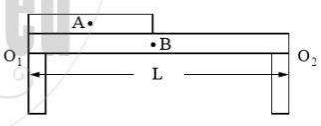
\includegraphics[width=0.4\linewidth]{../figs/VN10-2022-PH-TP022-P-1}
		\captionof{figure}{}
		\label{fig:23.8}
	\end{center}
	\begin{enumerate}[label=\alph*)]
		\item Xác định hợp lực của trọng lực tác dụng lên hai thanh dầm.
		\item Hai thanh dầm được đặt lên các cột đỡ tại $O_1$ và $O_2$. Để hệ đứng yên thì hợp lực $\vec F$ của các lực đỡ bởi hai cột phải cân bằng với hợp lực $\vec P$ xác định ở câu a. Hỏi mỗi cột đỡ chịu một lực bằng bao nhiêu?
	\end{enumerate}
}
\hideall{
	\begin{enumerate}[label=\alph*)]
		\item Áp dụng quay tắc hợp lực song song, cùng chiều cho hai trọng lực $\vec P_1$ và $\vec P_2$ của hai thanh, ta xác định được hợp lực $\vec P$:
		\begin{center}
			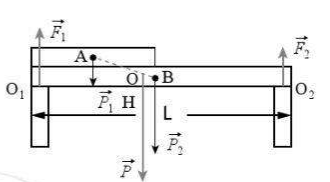
\includegraphics[width=0.4\linewidth]{../figs/VN10-2022-PH-TP022-P-2}
		\end{center}
		\begin{itemize}
			\item Độ lớn $P=P_1+P_2=\SI{15}{\kilo\newton}$.
			\item Giá của $\vec P$ đi qua điểm O chia đoạn AB theo tỉ lệ:
			$$\dfrac{OA}{OB}=\dfrac{P_2}{P_1}=\dfrac{10}{5}=2$$
			Mà khoảng cách giữa giá của $\vec P_1$ và $\vec P_2$ là $\dfrac{L}{4}$ nên khoảng cách từ giá của $\vec P$ đến giá của $\vec P_1$ và $\vec P_2$ lần lượt là $\dfrac{L}{6}$ và $\dfrac{L}{12}$.
		\end{itemize}
	\item Hợp lực $\vec F$ của các lực đỡ bởi hai cột phải cân bằng với $\vec P$, tức là:
	$F=P=\SI{15}{\kilo\newton}$, $\vec F$ ngược chiều và có giá trùng với giá của $\vec P$.\\
	Vì $\vec F$ là hợp lực của hai lực đỡ $\vec F_1$ và $\vec F_2$ song song, cùng chiều nên:
	\begin{align*}
		\begin{cases}
			F_1+F_2=F=\SI{15}{\kilo\newton}\\
			\dfrac{F_1}{F_2}=\dfrac{O_2H}{O_1H}=\dfrac{7}{5}
		\end{cases}
	\end{align*}
	Lực đỡ mỗi cột phải chịu:
	$$F_1=\SI{8.75}{\kilo\newton}; \quad F_2=\SI{6.25}{\kilo\newton}.$$
	\end{enumerate}
	
}

\item \mkstar{4}\\
{Một đĩa tròn phẳng, mỏng, đồng chất, bán kính $R$ sẽ có điểm đặt của trọng lực tại tâm của đĩa. Hỏi khi khoét một lỗ tròn bán kính $\dfrac{R}{2}$ thì trọng tâm của đĩa sẽ ở vị trí nào?
	\begin{center}
		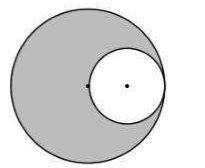
\includegraphics[width=0.2\linewidth]{../figs/VN10-2022-PH-TP022-P-3}
	\end{center}

}
\hideall{
Trọng tâm của đĩa bị khoét là điểm đặt hơp lực của trọng lực $P_K$ của hình tròn tâm K bán kính $\dfrac{R}{2}$ và trọng lực $P_I$ của phần đĩa còn lại sau khi khoét đi hai lỗ tròn đối xứng qua I.
\begin{center}
	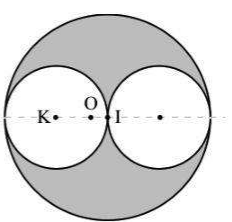
\includegraphics[width=0.2\linewidth]{../figs/VN10-2022-PH-TP022-P-4}
\end{center}
Vì đĩa phẳng đồng chất nên trọng lượng mỗi phần đĩa tỉ lệ với diện tích. Gọi $P$ là trọng lượng của đĩa nguyên, ta có:
$$\dfrac{P_K}{P}=\dfrac{\pi\left(\dfrac{R}{2}\right)^2}{\pi R^2}=\dfrac{1}{4}\Rightarrow P_K=\dfrac{P}{4}$$
Áp dụng quy tắc tổng hợp lực song song cùng chiều cho các trọng lực $P_I$ và $P_K$, ta xác định được điểm đặt O của hợp lực sẽ chia đoạn IK theo tỉ lệ:
$$\dfrac{OI}{OK}=\dfrac{P_K}{P_I}=\dfrac{\dfrac{P}{4}}{\dfrac{P}{2}}=\dfrac{1}{2}\Rightarrow OI=\dfrac{R}{6}.$$
}
\end{enumerate}